%%%%%%%%%%%%%%%%%%%%%%%%%%%%%%%%%%%%%%%%%
% Short Sectioned Assignment
% LaTeX Template
% Version 1.0 (5/5/12)
%
% This template has been downloaded from:
% http://www.LaTeXTemplates.com
%
% Original author:
% Frits Wenneker (http://www.howtotex.com)
%
% License:
% CC BY-NC-SA 3.0 (http://creativecommons.org/licenses/by-nc-sa/3.0/)
%
%%%%%%%%%%%%%%%%%%%%%%%%%%%%%%%%%%%%%%%%%

%----------------------------------------------------------------------------------------
%	PACKAGES AND OTHER DOCUMENT CONFIGURATIONS
%----------------------------------------------------------------------------------------

\documentclass[paper=a4, fontsize=11pt]{scrartcl} % A4 paper and 11pt font size
\usepackage[top=1in, bottom=1.5in, left=1in, right=1in]{geometry}
\usepackage{fancyhdr} % Required for custom headers
\usepackage{lastpage} % Required to determine the last page for the footer
\usepackage{extramarks} % Required for headers and footers
\usepackage[usenames,dvipsnames]{color} % Required for custom colors
\usepackage{graphicx} % Required to insert images
\usepackage{listings} % Required for insertion of code
\usepackage{courier} % Required for the courier font
\usepackage{amsmath}
\usepackage[super]{nth}
\usepackage{booktabs}
\usepackage[usenames,dvipsnames]{xcolor}
\usepackage{tcolorbox}
\usepackage{tabularx}
\usepackage{array}
\usepackage{colortbl}

%\usepackage[T1]{fontenc} % Use 8-bit encoding that has 256 glyphs
%\usepackage{fourier} % Use the Adobe Utopia font for the document - comment this line to return to the LaTeX default
\usepackage[english]{babel} % English language/hyphenation
\usepackage{amsmath,amsfonts,amsthm} % Math packages
\usepackage{graphicx}

\usepackage{hyperref}
\hypersetup{
  colorlinks   = true, %Colours links instead of ugly boxes
  urlcolor     = blue, %Colour for external hyperlinks
  linkcolor    = blue, %Colour of internal links
  citecolor   = red %Colour of citations
}

\usepackage{fancyhdr} % Custom headers and footers
\pagestyle{fancyplain} % Makes all pages in the document conform to the custom headers and footers
\fancyhead{} % No page header - if you want one, create it in the same way as the footers below
\fancyfoot[L]{} % Empty left footer
\fancyfoot[C]{} % Empty center footer
\fancyfoot[R]{\thepage} % Page numbering for right footer
\renewcommand{\headrulewidth}{0pt} % Remove header underlines
\renewcommand{\footrulewidth}{0pt} % Remove footer underlines
\setlength{\headheight}{13.6pt} % Customize the height of the header
\newcommand{\ts}{\textsuperscript}

\numberwithin{equation}{section} % Number equations within sections (i.e. 1.1, 1.2, 2.1, 2.2 instead of 1, 2, 3, 4)
\numberwithin{figure}{section} % Number figures within sections (i.e. 1.1, 1.2, 2.1, 2.2 instead of 1, 2, 3, 4)
\numberwithin{table}{section} % Number tables within sections (i.e. 1.1, 1.2, 2.1, 2.2 instead of 1, 2, 3, 4)

\setlength\parindent{0pt} % Removes all indentation from paragraphs - comment this line for an assignment with lots of text

% Default fixed font does not support bold face
\DeclareFixedFont{\ttb}{T1}{txtt}{bx}{n}{8} % for bold
\DeclareFixedFont{\ttm}{T1}{txtt}{m}{n}{8}  % for normal

%----------------------------------------------------------------------------------------
%	CODE BLOCKS
%----------------------------------------------------------------------------------------

\usepackage{adjustbox}
\usepackage{listings}
\usepackage{color}

\definecolor{dkgreen}{rgb}{0,0.6,0}
\definecolor{gray}{rgb}{0.5,0.5,0.5}
\definecolor{mauve}{rgb}{0.58,0,0.82}

\lstdefinelanguage{Dockerfile}
{
  morekeywords={FROM, RUN, CMD, LABEL, MAINTAINER, EXPOSE, ENV, ADD, COPY,
    ENTRYPOINT, VOLUME, USER, WORKDIR, ARG, ONBUILD, STOPSIGNAL, HEALTHCHECK,
    SHELL},
  morecomment=[l]{\#},
  morestring=[b]"
}

\lstset{
    columns=flexible,
    aboveskip=5mm,
    belowskip=5mm,
    keepspaces=true,
    showstringspaces=false,
    basicstyle=\ttfamily,
    commentstyle=\color{gray},
    keywordstyle=\color{purple},
    stringstyle=\color{green}
}



%----------------------------------------------------------------------------------------
%	TITLE SECTION
%----------------------------------------------------------------------------------------

\usepackage{eso-pic}
% \usepackage[demo]{graphicx}
\newcommand\AtPageUpperRight[1]{\AtPageUpperLeft{%
   \makebox[\paperwidth][r]{#1}}}

\newcommand{\horrule}[1]{\rule{\linewidth}{#1}} % Create horizontal rule command with 1 argument of height

\title{	
\normalfont \normalsize
\textsc{Northeastern University,  Khoury College of Computer Science} \\ [25pt] % Your university, school and/or department name(s)
\horrule{0.5pt} \\[0.4cm] % Thin top horizontal rule
\huge CS 6220  Data Mining \textemdash~Assignment 1\\ % The assignment title
\Large \textbf{Due: January 18, 2022 (100 points)} % The assignment title
\horrule{2pt} \\[0.5cm] % Thick bottom horizontal rule
}

\author{\textbf{YOUR NAME} \\ \textbf{YOUR LDAP}} % Your name

\date{} % Today's date or a custom date

\begin{document}

\AddToShipoutPictureBG*{%
  \AtPageUpperRight{\raisebox{-\height}{
\includegraphics[width=3cm]{images/logo}}}}
\maketitle % Print the title

%%%%%%%%%%%%%%%%%%%%
\section{Getting Started - 10 points}
%%%%%%%%%%%%%%%%%%%%
\subsection{Using Docker}


Different companies use different tools for development and different work environments. For future assignments, we won't be prescriptive, but in this homework, we're going to familiarize ourselves with some of the most useful and common delivery and development environment tools in industry today.

Docker \url{http://www.Docker.com} is a  useful mechanism for delivering software or scaling it up. For example, say we want to run a multi-computer job, passing \emph{Docker containers} to each of the nodes in the cluster is one way to have repetitive and predictable behavior when doing large scale compute.

There are two essential Docker units: a \textbf{container} and a \textbf{container image}.

\begin{enumerate}
    \item A \textbf{container} is a sandboxed process on your machine that is isolated from all other processes on the host machine. That isolation leverages kernel namespaces and cgroups, features that have been in Linux for a long time. Docker has worked to make these capabilities approachable and easy to use. To summarize, a container:
    \begin{enumerate}
        \item is a runnable instance of an image. You can create, start, stop, move, or delete a container using the DockerAPI or CLI. 
        \item can be run on local machines, virtual machines or deployed to the cloud.
        \item is portable (can be run on any OS).
        \item is isolated from other containers and runs its own software, binaries, and configurations.
    \end{enumerate}

    \item When running a container, it uses an isolated filesystem. This custom filesystem is provided by a \textbf{container image}. Since the image contains the container’s filesystem, it must contain everything needed to run an application - all dependencies, configurations, scripts, binaries, etc. The image also contains other configuration for the container, such as environment variables, a default command to run, and other metadata.
\end{enumerate}

Go ahead and download and install Docker. The getting started guide on Docker has detailed instructions for setting up Docker on 
\begin{itemize}
    \item Mac \url{https://docs.docker.com/desktop/install/mac-install/},
    \item Linux \url{https://docs.docker.com/install/linux/docker-ce/ubuntu}
    \item Windows \url{https://docs.docker.com/docker-for-windows/install}.
\end{itemize}

\subsection{Executing Your ``Hello World''}

For this assignment, we'll start with creating a Dockerfile in your submission folder. Specify the operating system and version of Python in the Dockerfile. You will subsequently need to install Python and libraries that you anticipate importing. Do not add the data into the image; you will need to pass that into the container with the \verb"-v" Docker option.

% Taken from 
% https://www.codewithjason.com/docker-hello-world-app/

For example, here's the most basic \verb"Dockerfile":

\begin{lstlisting}[language=Dockerfile]
FROM ubuntu:20.04

RUN apt update && apt install -y sbcl
WORKDIR /usr/src
\end{lstlisting}

For this assignment, you'll set up your Docker environment and the appropriate versions of Python. Specifically,

\begin{enumerate}
    \item Download and install Docker
    \item Create your Dockerfile
    \item Compile your Docker image
    \item Screenshot a list of the Docker images available
    \item Screenshot a list of the running Docker containers that include one with the image you created
    \item Include both screenshots and the command you used in your write up
\end{enumerate}

%%%%%%%%%%%%%%%%%%%%
\subsection{Github}
%%%%%%%%%%%%%%%%%%%%

Software version control at companies is essential for every software company in the industry. There are several types, including \emph{Subversion/SVN} (which Google uses its in-house version branched from SVN). The most popular tool of choice is Github, which Microsoft recently bought. 

At the end of this assignment, your submission will point to a repository, where the following files will be reviewed and subsequently graded:

\begin{itemize}
    \item \verb"Dockerfile" specifying what packages that you've used
    \item \verb"assignment1.tex" file with your homework writeup
    \item \verb"assignment1.pdf" file of the compiled version of your *.tex file
    \item \verb"assignment1.py" file of your working code
\end{itemize}

None of the other files in that repository will be reviewed. We've provided a \LaTeX template that you can use for submission, provided here:
\begin{itemize}
    \item \url{https://github.com/kni-neu/homework-1/blob/main/assignment1_template.tex}
\end{itemize}

Do \emph{NOT} include data into your Git repository.

%%%%%%%%%%%%%%%%%%%%
\section{Identifying All Sets - 40 points}
%%%%%%%%%%%%%%%%%%%%

In subsequent lectures, you'll learn about frequent item sets, where relationships between items are learned by observing how often they co-occur in a set of data. This information is useful for making recommendations in a rule based manner. Before looking at frequent item sets, it is worth understanding the space of all possible sets and get a sense for how quickly the number of sets with unique items grows.

Suppose that we've received only a hundred records of items bought by customers at a market. Each line in the file represents the items an individual customer bought, i.e. their basket. For example, consider the following rows.

\begin{lstlisting}
ham, cheese, bread
dates, bananas
celery, chocolate bars
\end{lstlisting}

Customer 1 has a basket of ham, cheese, and bread. Customer 2 has a basket of dates and bananas. Customer 3 has a basket of celery and chocolate bars. Each of these records is the receipt of a given customer, identifying what they bought.

\begin{enumerate}
    \item What is the cardinality of the full set of unique items? Write a function called \verb"cardinality_items" that takes a \verb".csv" text string file as input, where the format is as the above, and calculates the cardinality of the dataset.
    \item Taking any \verb".csv" file as a sample of a larger dataset, we'd occasionally like to understand the space of all possible subsets comprised of unique items. If there are $N$ unique items (i.e., the cardinality of the entire dataset is $N$), how many sets with unique items can there possibly be? (Ignore the null set.)
    \item Write a module called \verb"all_itemsets()" with the following input/output:
      \begin{enumerate}
      \item Input: $filename$ = the \verb".csv" text string file, where the format is as the above.
      \item Output: $L = [ S_1, S_2, \cdots S_N ]$ = A list of all possible sets of size $N$
      \end{enumerate}
    \item Let's take the small sample \verb".csv" provided as reflective of the distribution of the receipts writ large. So, for example, if the set $S= \{ \text{bread}, \text{oatmeal}\}$ occurs twice in a dataset with $100$ records, then the probability of item set $\{ \text{bread}, \text{oatmeal} \}$ occurring is 0.02. Write a module called \verb"prob_S" with the following input/output:
      \begin{enumerate}
      \item Input: \\ $S$ = the set in question \\ $D$ = the entire Dataset (which if it's in memory, Python will pass by reference)
      \item Output: $P(S)$ = the probability that $S$ occurs
      \end{enumerate}
\end{enumerate}


%%%%%%%%%%%%%%%%%%%%
\section{The Netflix Challenge - 50 points}
%%%%%%%%%%%%%%%%%%%%

One of the most famous challenges in data science and machine learning is Netflix's Grand Prize Challenge, where Netflix held an open competition for the best algorithm to predict user ratings for films. The grand prize was \$1,000,000 and was won by BellKor's Pragmatic Chaos team. 

This is the dataset that was used in that competition.
\begin{itemize}
    \item \url{https://www.kaggle.com/datasets/netflix-inc/netflix-prize-data}
\end{itemize}

In this exercise, we're going to do a bit of exploring in the Netflix Data. Start by downloading the data. If all worked out well, you should have the files in Fig.~\ref{fig:data-files}. The Kaggle dataset is close to 700MB large, and may take a long time to download. Do \emph{not} include this data in your Docker container, but rather, mount the folder with the data.

%%%%%%%%%%%%%%%%%%%%
\subsection{Data Verification}
%%%%%%%%%%%%%%%%%%%%

Data integrity tends to be a problem in large scale processing, especially if there is little to no support. Therefore, it's important to verify the quality of the file download. 

\noindent
\begin{enumerate}
\item A large part of machine learning and data science is about getting data in the right format. Verify that the schema is the same as the Kaggle Dataset's description. Add screenshots to your assignment.
\end{enumerate}


%%%%%%%%%%%%%%%%%%%%
\subsection{Data Analysis}
\label{sec:data-analysis}
%%%%%%%%%%%%%%%%%%%%

Let's answer the following questions in your writeup: 

\begin{enumerate}
    \item How many total records are there?
    \item Can you plot the distribution of star ratings over users and time? The granularity of the sliding window is at your discretion. Are there any trends?
    \item What percentage of the films have gotten \emph{more} popular over time?
    \item How many films have been re-released? How do you know?
    \item What other information might we try to extract to better understand the data? For the questions that you may come up with (especially any time series data), make sure you back up your assertions with plots. Go ahead and play around with the data, and explore. 
    \item What are some interesting problems that we might solve? (No need to actually solve them!)
\end{enumerate}

\begin{figure}
    \centering
    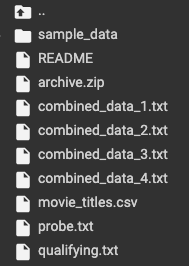
\includegraphics{images/hw1q2.png}
    \caption{If everything worked out well, you should have the above files available to browse and process.}
    \label{fig:data-files}
\end{figure}

\section{Grading Criterion}

A significant portion of the grading rubric is the presentation of your report. We'll review:

\begin{enumerate}
    \item the answers to questions.
    \item your code and its legibility
    \item the clarity of your write-up, including 
    \begin{enumerate}
      \item pipeline and code decisions, 
      \item perspectives on the solution, 
      \item and algorithmic rationale.
    \end{enumerate}
\end{enumerate}


\end{document}
